\documentclass[conference]{IEEEtran}
\IEEEoverridecommandlockouts
% The preceding line is only needed to identify funding in the first footnote. If that is unneeded, please comment it out.
% \usepackage{cite}
\usepackage{cite}
\usepackage{amsmath,amssymb,amsfonts}
\usepackage{algorithmic}
\usepackage{graphicx}
\graphicspath{ {./images/} }
\usepackage{textcomp}
\usepackage{tikz}
\usepackage{pgfplots}
\usepackage{xcolor}
\usepackage{caption}  

% biblatex
% \usepackage{biblatex}
% \addbibresource{bibtex/PaperDubai.bib}
% \addbibresource{zotero.bib}

\def\BibTeX{{\rm B\kern-.05em{\sc i\kern-.025em b}\kern-.08em
    T\kern-.1667em\lower.7ex\hbox{E}\kern-.125emX}}
\begin{document}

\makeatletter
\newcommand{\linebreakand}{%
    \end{@IEEEauthorhalign}
    \hfill\mbox{}\par
    \mbox{}\hfill\begin{@IEEEauthorhalign}
}
\makeatother

\title{Performance comparison of natural language understanding services in the educational domain}

\author{\IEEEauthorblockN{1\textsuperscript{st} Víctor Juan Jimenez Flores}
    \IEEEauthorblockA{\
        % textit{dept. name of organization (of Aff.)} \\
        \textit{Universidad José Carlos Mariátegui}\\
        Tacna, Perú \\
        victorjuanjf@jfbots.com}
    % asociación peruana de investigación, ciencia y tecnología comprar dominio antes de enviar paper
    \and
    \IEEEauthorblockN{2\textsuperscript{nd} Oscar Juan Jimenez Flores}
    \IEEEauthorblockA{
        % \textit{dept. name of organization (of Aff.)} \\
        \textit{Universidad Privada de Tacna}\\
        Tacna, Perú \\
        oscarjimenezflores@upt.pe}
    \and
    \IEEEauthorblockN{3\textsuperscript{rd} Juan Carlos Jimenez Flores}
    \IEEEauthorblockA{
        % \textit{dept. name of organization (of Aff.)} \\
        \textit{Southern Perú Copper Corporation}\\
        Tacna, Perú \\
        juancarlosjf@apicyt.com}
    \linebreakand % <------------- \and with a line-break
    \IEEEauthorblockN{4\textsuperscript{th} Juan Ubaldo Jimenez Castilla}
    \IEEEauthorblockA{
        % \textit{dept. name of organization (of Aff.)} \\
        \textit{Universidad José Carlos Mariátegui }\\
        Moquegua, Perú \\
        jjimenezc@ujcm.edu.pe}
}

\maketitle

\begin{abstract}
    The research aims to compare the main natural language understanding (NLU) services and determine which one has the highest performance in the educational domain. In this study, six NLU services were compared and performance was measured with the F1 score. Moreover, training data and input messages were extracted from Mariateguino Bot,which was the chatbot of the José Carlos Mariátegui University during 2018.
\end{abstract}

\begin{IEEEkeywords}
    chatbot, Natural Language Understanding, NLU, F1 score, performance
\end{IEEEkeywords}

\section{Introduction}
Nowadays, the industry and researchers are increasingly recognize the importance of chatbot systems, because they are integrated into everyday life, playing roles as assistants to end users \cite{Bird2018}. A chatbot is a computer program which uses machine learning technique voice recognition, and natural language processing (NLP) to conduct a intelligent conversation with a person (e.g. Amazon's Alexa and Google's Assistant) \cite{mittal2019getting}. Moreover, one of the main components of a chatbot is the natural language understanding (NLU), which is the ability of a machine to understand human languages, said otherwise, it is the process of converting natural language text into a form that computers can understand \cite{pathak2017artificial}.

Throughout this paper, the term NLU

Previous work has only focused on

In this research, the performance of six NLU services was evaluated

This paper is divided into five sections. Section II gives a brief overview of related works. The third section defines the NLU services evaluated during the research.

Training data and input messages were extracted from Mariateguino Bot,which was the chatbot of the José Carlos Mariátegui University during 2018, its main function was to attend to the doubts of the students regarding the necessary requirements to carry out administrative procedures. Moreover, the chatbot was able to answer frequently asked questions, support students regarding the admissions process, and provide class schedules.

Mariateguino Bot was made with Dialogflow \cite{dialogflow2020}, a Google service that runs on Google Cloud Platform. Therefore, other platforms, described in section \ref{sec:nluServices}, were evaluated.

In order to identify F1 score, it was necessary to calculate the precision and recall.

The F1 score was chosen beacuse it is one of the most practical ways to numerically calculate the performance of an NLU service

\section{Related works}
In recent years, multiple investigations have been carried out regarding chatbots and the impact they have on traditional processes, generally in customer service. Some of these researches are listed below.

Canonico and De Russis wrote a paper titled "A comparison and Critique of Natural Language Understanding Tools" \cite{Canonico2018}, which compares the main cloud-based platforms, from a descriptive and performance based point of view. Their results showed that Watsson Assistant is the platform who performs best.

In the other hand, Braun, Hernandez, Matthes and Langen wrote a paper titles "Evaluating Natural Language Understanding Services for Conversational Question Answering Systems", which presents a method to evaluate the classification performance of NLU services. Their results indicated that LUIS showed the best scores and RASA could achieve similar results.

\section{Natural language understanding services} \label{sec:nluServices}
There are many natural language understanding modules that are available as cloud services and major IT players like Google, Microsoft, IBM, Facebook and Amazon have created tools to develop chatbots \cite{hall2017hands}. Additionally, Rasa was included because Dialogflow training data can be converted to its format and is an open source alternative compared to  the other platforms.
\subsection{Dialogflow}
Dialogflow is a Google service that runs on Google Cloud Platform. Dialogflow is a natural language understanding platform that makes it easy to design and integrate a conversational user interface into any system \cite{dialogflow2020}.
\subsection{LUIS}
The Language Understanding Intelligent Service (LUIS) is a Microsoft's NLU cloud service and is part of the cognitive suite \cite{pathak2018iot}.
\subsection{Watsson Assistant}
Watsson Assistant is a cognitive cloud service offering by IBM that makes it easier for developers to build conversational interfaces and embed them into any application \cite{sabharwal2019developing}.
\subsection{Wit.ai}
Facebook has established the Wit.ai bot engine which allows training bots with sample conversations and have your bots repeatedly learn from interrelating with customers \cite{seligman2018artificial}.
\subsection{Amazon LEX}
Amazon Lex is a development platform, belonging to Amazon, for building intelligent assistants or chatbots, which provides many AI capabilities like Automatic Speech Recognition (ASR) and Natural language Understanding (NLU) \cite{tripuraneni2019hands}.
\subsection{Rasa}
Rasa NLU is an open-source NLP library for intent classification and entity extraction in chatbots \cite{raj2018building}.

\section{Methods}
The method of evaluating the classification performance of NLU services is based on \cite{Braun2017}.
\subsection{Materials}
The NLU services evaluated during the research were Dialogflow, Wit.ai, LUIS, Amazon LEX and Rasa. Moreover, 100 messages from the Mariateguino Bot conversation history were selected as input data and they were grouped based on the expected intents, thus obtaining 30 intents. To calculate the performance of each platform, the F1 score metric was used, which includes precision and recall.

\subsection{Procedure}
The experimental design , indicated below, is based on \cite{Braun2017}.

As a first step, a conversion of the Dialogflow training data to the rest of the research platforms was carried out, using the QBox.ai service \cite{qbox2020}. Then, one hundred messages were randomly selected from Mariateguino Bot conversation history and they were grouped based on the expected intents, thus obtaining 30 intents.

Afterwards, to start testing and obtain data, a Node.js application was created in order to combine the application programming interface (API) from each NLU service, in such a way that each input message was only entered once and the desired data was obtained in the format shown in Fig. \ref{fig:nludata}. Also, a threshold of 0.5 was programmed for all platforms, so that if the API of the NLU service returns a confidence less than 0.5, the Node.js application returns the default fallback intent.

\begin{figure}[htbp]
    \centerline{\fbox{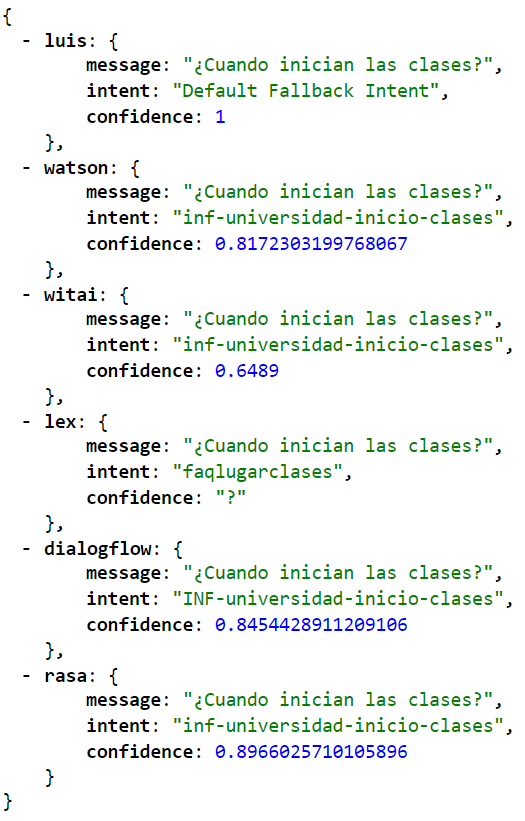
\includegraphics[scale=0.58]{nlu}}}
    \caption{Node.js application output}
    \label{fig:nludata}
\end{figure}

In order to evaluate the results, the predicted intent were identified for each input message. In this way, true positives (TP), false positives (FP) and false negatives (FN) were calculated.

As a final step, the performance of the NLU services was measure in terms of precision, recall and F1 score, given by the following expressions:

\begin{equation}
    Precision=\frac{TP}{TP+FP}\label{eq1}
\end{equation}
\begin{equation}
    Recall=\frac{TP}{TP+FN}\label{eq2}
\end{equation}
F1 score is defined as the harmonic mean of precision and recall \cite{campesato2020artificial}.
\begin{equation}
    F_{1} =\frac{2 \times Precision\times Recall}{Precision+Recall}\label{eq3}
\end{equation}

These measures were applied for single intents, then the average F1 score was calculated. For this research, one NLU service is better than another if it has a higher average F1 score.

\section{Results}

The results shown in Fig. \ref{fig:precision}, Fig. \ref{fig:recall}, Fig. \ref{fig:f1score} and table \ref{tab:overview} are the average f1 score of the 30 intents that were evaluated for each natural language understanding service

In terms of precision, as Fig. \ref{fig:precision} shows, Dialogflow has the highest value, while LUIS obtained the lowest value.

In terms of recall, as Fig. \ref{fig:precision} shows, Dialogflow has the highest value, while LUIS obtained the lowest value.

Finally, in terms of precision, as Fig. \ref{fig:precision} shows, Dialogflow has the highest value, while LUIS obtained the lowest value.

Overall, as can be seen in the table \ref{tab:overview}, Watson Assistant performed better in terms of F1 score, while LUIS obtained the lowest performance.

\begin{figure}[htbp]
    \begin{center}
        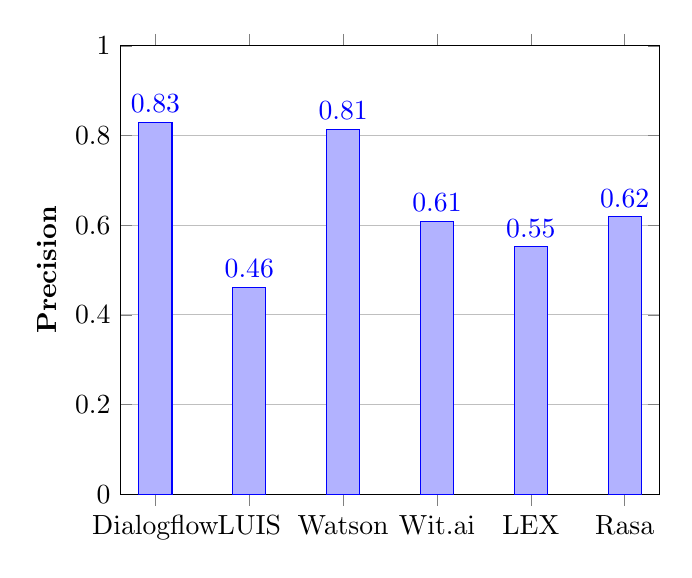
\begin{tikzpicture}
            \begin{axis}
                [
                    ybar,
                    bar width=12pt,
                    ylabel=Precision,
                    % xlabel=NLU services,
                    symbolic x coords={Dialogflow,LUIS,Watson,Wit.ai,LEX,Rasa},
                    enlarge x limits=0.075,
                    xtick=data,
                    xmajorgrids = false,
                    ymajorgrids = true,
                    ymin=0,
                    ymax=1,
                    % axis y line = left,
                    every outer y axis line/.append style = {-},
                    every outer x axis line/.append style = {-},
                    ylabel style = {font=\bfseries},
                    xlabel style = {font=\bfseries},
                    nodes near coords,
                    nodes near coords align={vertical},
                ]
                \addplot coordinates {(Dialogflow,0.828333333) (LUIS,0.461717171717172) (Watson,0.813918128654971) (Wit.ai,0.607663117663118) (LEX,0.551633986928105) (Rasa,0.618515325670498) };
            \end{axis}
        \end{tikzpicture}
        \captionof{figure}{Precision of natural language understanding services}
        \label{fig:precision}
    \end{center}
\end{figure}
\begin{figure}[htbp]
    \begin{center}
        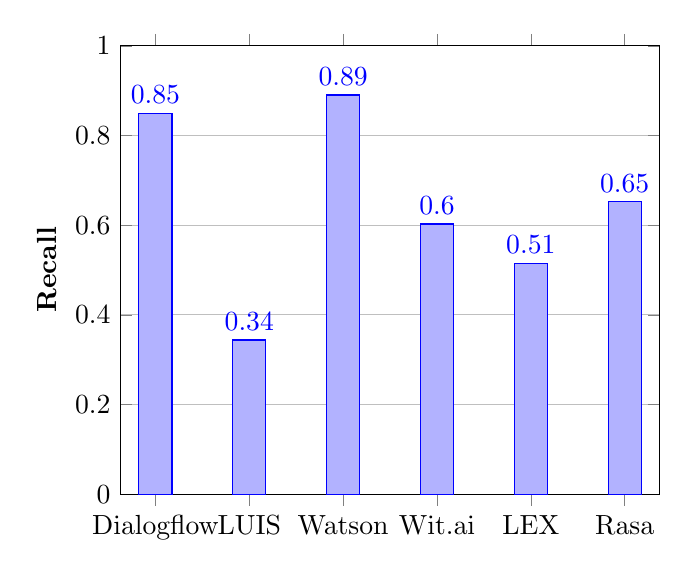
\begin{tikzpicture}
            \begin{axis}
                [
                    ybar,
                    bar width=12pt,
                    ylabel=Recall,
                    % xlabel=NLU services,
                    symbolic x coords={Dialogflow,LUIS,Watson,Wit.ai,LEX,Rasa},
                    enlarge x limits=0.075,
                    xtick=data,
                    xmajorgrids = false,
                    ymajorgrids = true,
                    ymin=0,
                    ymax=1,
                    % axis y line = left,
                    every outer y axis line/.append style = {-},
                    every outer x axis line/.append style = {-},
                    ylabel style = {font=\bfseries},
                    xlabel style = {font=\bfseries},
                    nodes near coords,
                    nodes near coords align={vertical},
                ]
                \addplot coordinates {(Dialogflow,0.848744588744589) (LUIS,0.343726551226551) (Watson,0.89017316017316) (Wit.ai,0.602640692640693) (LEX,0.514170274170274) (Rasa,0.651991341991342) };
            \end{axis}
        \end{tikzpicture}
        \captionof{figure}{Recall of natural language understanding services}
        \label{fig:recall}
    \end{center}
\end{figure}
\begin{figure}[htbp]
    \begin{center}
        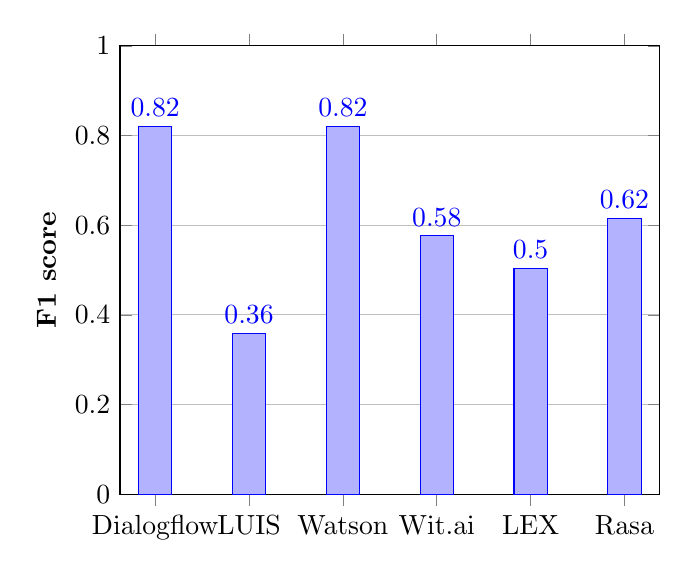
\begin{tikzpicture}
            \begin{axis}
                [
                    ybar,
                    bar width=12pt,
                    ylabel=F1 score,
                    % xlabel=NLU services,
                    symbolic x coords={Dialogflow,LUIS,Watson,Wit.ai,LEX,Rasa},
                    enlarge x limits=0.075,
                    xtick=data,
                    xmajorgrids = false,
                    ymajorgrids = true,
                    ymin=0,
                    ymax=1,
                    % axis y line = left,
                    every outer y axis line/.append style = {-},
                    every outer x axis line/.append style = {-},
                    ylabel style = {font=\bfseries},
                    xlabel style = {font=\bfseries},
                    nodes near coords,
                    nodes near coords align={vertical},
                ]
                \addplot coordinates {(Dialogflow,0.820630111) (LUIS,0.357854738
                        ) (Watson,0.820979481) (Wit.ai,0.576004394) (LEX,0.503356458) (Rasa,0.615315904) };
            \end{axis}
        \end{tikzpicture}
    \end{center}
    \captionof{figure}{F1 score of natural language understanding services}
    \label{fig:f1score}
\end{figure}

\begin{table}[htbp]
    \caption{F1 scores overview erge}
    \begin{center}
        \begin{tabular}{|c|c|c|c|}
            \hline
            \textbf{NLU Service} & \textbf{Precision} & \textbf{Recall} & \textbf{F1 score} \\
            \hline
            Dialogflow           & 0.83               & 0.85            & 0.82              \\
            \hline
            LUIS                 & 0.46               & 0.34            & 0.35              \\
            \hline
            Watson               & 0.81               & 0.89            & 0.82              \\
            \hline
            Wit.ai               & 0.61               & 0.60            & 0.58              \\
            \hline
            LEX                  & 0.55               & 0.51            & 0.50              \\
            \hline
            RASA                 & 0.62               & 0.65            & 0.62              \\
            \hline
        \end{tabular}%
        \label{tab:overview}%
    \end{center}
\end{table}%
\section{Discussion}

Previous researches

Despite the fact that Watson Assistant and Dialogflow obtained the same F1 score, Watson Assistant can be considered performed   best because the original service with which the chatbot was in production was Dialogflow, so it was constantly improving only on that service.

On the other hand, the lower performance of LUIS may be due to the language. Mariateguino Bot was a chatbot made for students in the Spanish language and, despite the fact that LUIS has Spanish in its configuration, it was observed that the intent classification decreases considerably in the presence of input messages that have words with a Spanish accent.

\section{Conclusion}
The objective of this research was to compare the main natural language understanding services and determine which one has the highest performance in the educational domain.
\section{Future work}

\section*{Acknowledgment}

The preferred spelling of the word ``acknowledgment'' in America is without
an ``e'' after the ``g''. Avoid the stilted expression ``one of us (R. B.
G.) thanks $\ldots$''. Instead, try ``R. B. G. thanks$\ldots$''. Put sponsor
acknowledgments in the unnumbered footnote on the first page.

\bibliographystyle{IEEEtran}
% \printbibliography
\bibliography{C:/Users/JIMENEZ/Documents/bibtex/PaperIEEE.bib}

\end{document}